% !Mode:: "TeX:UTF-8"
\documentclass[openany]{book}
% !Mode:: "TeX:UTF-8"
\usepackage[english]{babel}
\usepackage[UTF8]{ctex}
\usepackage{amsmath, amsthm, amssymb}

% Figure
\usepackage{graphicx}
\usepackage{float} %% H can fix the location
\usepackage{caption}
\usepackage[format=hang,singlelinecheck=0,font={sf,small},labelfont=bf]{subfig}
\usepackage[noabbrev]{cleveref}
\captionsetup[subfigure]{subrefformat=simple,labelformat=simple,listofformat=subsimple}
\renewcommand\thesubfigure{(\alph{subfigure})}

\usepackage{epstopdf} %% convert eps to pdf
\DeclareGraphicsExtensions{.eps,.mps,.pdf,.jpg,.png} %% bmp, gif not supported
\DeclareGraphicsRule{*}{eps}{*}{}
\graphicspath{{img/}{figure/}{../figure/}} %% fig directorys

%% \usepackage{pstricks} %% a set of macros that allow the inclusion of PostScript drawings directly inside TeX or LaTeX code
%% \usepackage{wrapfig} %% Wrapping text around figures

% Table
\usepackage{booktabs} %% allow the use of \toprule, \midrule, and \bottomrule
\usepackage{tabularx}
\usepackage{multirow}
\usepackage{colortbl}
\usepackage{longtable}
\usepackage{supertabular}

\usepackage[colorinlistoftodos]{todonotes}

% Geometry
\usepackage[paper=a4paper, top=1.5cm, bottom=1.5cm, left=1cm, right=1cm]{geometry}
%% \usepackage[paper=a4paper, top=2.54cm, bottom=2.54cm, left=3.18cm, right=3.18cm]{geometry} %% ms word
%% \usepackage[top=0.1cm, bottom=0.1cm, left=0.1cm, right=0.1cm, paperwidth=9cm, paperheight=11.7cm]{geometry} %% kindle

% Code
%% \usepackage{alltt} %% \textbf can be used in alltt, but not in verbatim

\usepackage{listings}
\lstset{
    backgroundcolor=\color{white},
    columns=flexible,
    breakatwhitespace=false,
    breaklines=true,
    captionpos=tt,
    frame=single, %% Frame: show a box around, possible values are: none|leftline|topline|bottomline|lines|single|shadowbox
    numbers=left, %% possible values are: left, right, none
    numbersep=5pt,
    showspaces=false,
    showstringspaces=false,
    showtabs=false,
    stepnumber=1, %% interval of lines to display the line number
    rulecolor=\color{black},
    tabsize=2,
    texcl=true,
    title=\lstname,
    escapeinside={\%*}{*)},
    extendedchars=false,
    mathescape=true,
    xleftmargin=3em,
    xrightmargin=3em,
    numberstyle=\color{gray},
    keywordstyle=\color{blue},
    commentstyle=\color{green},
    stringstyle=\color{red},
}

% Reference
%% \bibliographystyle{plain} % reference style

% Color
\usepackage[colorlinks, linkcolor=blue, anchorcolor=red, citecolor=green, CJKbookmarks=true]{hyperref}
\usepackage{color}
\def\red#1{\textcolor[rgb]{1.00,0.00,0.00}{#1}}
\newcommand\warning[1]{\red{#1}}

% Other
%% \usepackage{fixltx2e} %% for use of \textsubscript
%% \usepackage{dirtree}  %% directory structure, like the result of command tree in bash shell

   %导入需要用到的package
% !Mode:: "TeX:UTF-8"

% Chapter
%% \makeatletter\@addtoreset{chapter}{part}\makeatother %% have chapters numbered without interruption (numbering through parts)

% Equation
\makeatletter\@addtoreset{equation}{section}\makeatother 
\renewcommand\theequation{%
\thepart\arabic{chapter}%
-\thepart\arabic{section}%
-\thepart\arabic{equation}%
}

% Theorem
\newtheorem{definition}{D\'efintion}
\newtheorem*{thmwn}{Thm}
\newtheorem{theorem}{Th\'eor\`eme}[chapter]
\newtheorem{corollary}{Corollary}[theorem]
\newtheorem{lemma}{Lemma}
\newtheorem{proposition}{Proposition}[chapter]
\newtheorem*{attention}{Attention}
\newtheorem*{note}{Note}
\newtheorem*{remark}{Remark}
\newtheorem{example}{Example}
\newtheorem{question}{Question}[chapter]
\newtheorem{problem}{Problem}
\newtheorem*{answer}{Answer}
\newtheorem{fact}{Fact}

   %导入需要用到的package

\begin{document}
\title{Paper Reading Notes}
\author{Eric}
\maketitle
\tableofcontents
\frontmatter

\part{Computer}
M/M/1排队模型(M/M/1 model)是一种单一服务器(single-server)的(排队模型),可用作模拟不少系统的运作。
依据开恩特罗符号必须有下列的条件:
\begin{itemize}
\item 到达时间服从泊松分布(Poisson distribution)\ref{sec.distribution.poisson};
\item 服务时间是指数分布(exponentially distributed)\ref{sec.distribution.exponential};
\item 只有一部服务器(server)
\item 队列长度无限制
\item 可加入队列的人数为无限
\end{itemize}
\begin{figure}[htbp]
  \centering
  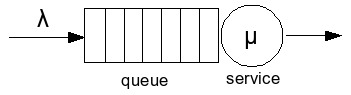
\includegraphics[scale = 0.3]{Mm1}\\
  \caption{Mm1}\label{fig.Mm1}
\end{figure}

这种模型是一种出生-死亡过程,此随机过程中的每一个状态代表模型中人数的数目。因为模型的队列长度无限且参与人数亦无限,故此状态数目亦为无限。例如状态0表示模型闲置、状态1表示模型有一人在接受服务、状态2表示模型有二人(一人正接受服务、一人在等候),如此类推。 此模型中,出生率(即加入队列的速率)$\lambda$ 在各状态中均相同,死亡率(即完成服务离开队列的速率)$\mu$亦在各状态中相同(除了状态0,因其不可能有人离开队列)。

故此,在任何状态下,只有两种事情可能发生:
\begin{itemize}
\item 有人加入队列。如果模型在状态k,它会以速率$\lambda$ 进入状态$k + 1$
\item 有人离开队列。如果模型在状态k(k不等于0),它会以速率$\mu$进入状态$k ? 1$
\end{itemize}
%% %% on the state space {0,1,2,3,...}. This is the same continuous time Markov chain as in a birth–death process. The state space diagram for this chain is as below.
\begin{tikzpicture}%[->,>=stealth',shorten >=1pt,auto,node distance=2cm,semithick]
  % \tikzstyle{every state}=[fill=white,draw=black,text=black,minimum size=1.1cm]
  \tikzstyle{state}=[fill=white,draw=black,text=black,minimum size=1.1cm]
 
  \node[state] (A) {0};
  \node[state] (B) [right of=A] {$1$};
  \node[state] (C) [right of=B] {$2$};
  \node[state] (D) [right of=C] {$3$};
  \node[minimum size=1cm] (E) [right of=D] {$\cdots$};
  \node[state] (F) [right of=E] {$n-1$};
  \node[state] (G) [right of=F] {$n$};
  \node[state] (H) [right of=G] {$n+1$};
  \node[minimum size=1cm] (I) [right of=H] {$\cdots$};
 
  \path (A) edge [bend left] node {$\lambda$} (B);
  \path (B) edge [bend left] node {$\mu$} (A);
  \path (B) edge [bend left] node {$\lambda$} (C);
  \path (C) edge [bend left] node {$\mu$} (B);
  \path (C) edge [bend left] node {$\lambda$} (D);
  \path (D) edge [bend left] node {$\mu$} (C);
  \path (D) edge [bend left] node {$\lambda$} (E);
  \path (E) edge [bend left] node {$\mu$} (D);
  \path (E) edge [bend left] node {$\lambda$} (F);
  \path (F) edge [bend left] node {$\mu$} (E);
  \path (F) edge [bend left] node {$\lambda$} (G);
  \path (G) edge [bend left] node {$\mu$} (F);
  \path (G) edge [bend left] node {$\lambda$} (H);
  \path (H) edge [bend left] node {$\mu$} (G);
  \path (H) edge [bend left] node {$\lambda$} (I);
  \path (I) edge [bend left] node {$\mu$} (H);
\end{tikzpicture}

\begin{figure}[htbp]
  \centering
  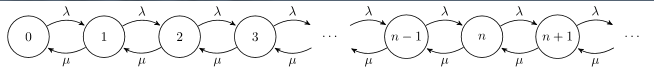
\includegraphics[scale = 0.5]{state_space}\\
  \caption{State space transmission}\label{fig.state_space}
\end{figure}

由此可见,模型的隐定条件为$\lambda < \mu$。如果死亡率小于出生率,则队列中的平均人数为无限大,故此这种系统没有平衡点。

此模型中有几项数值常被测量,例如:
\begin{itemize}
\item 一人在系统中的平均逗留时间
\item 一人在接受服务前的平均等候时间
\item 整个系统中的平均人数
\item 等候队列的平均人数
\item 一单位时间内系统完成服务人数,即服务速度
\end{itemize}

稳定状态下的公式

定义 $\scriptstyle \rho \,=\,{\tfrac  {\lambda }{\mu }}$.
则模型在状态i的机率为
$$
{\mbox{Prob}}(q=i)=\pi _{i}=(1-\rho )\rho ^{i}.\,
$$
由此,可给出各测量数值的公式:
整个系统的平均人数N:$\overline N={\frac  {\rho }{1-\rho }}$,
且其变异(variance)为$\sigma _{N}^{2}={\frac  {\rho }{(1-\rho )^{2}}}$.
一单位时间内系统完成服务的人数:$\overline N_{S}=\lambda \overline x=\rho$
在队列中等候服务的人数:$\overline N_{Q}={\frac  {\rho ^{2}}{1-\rho }}$
一人在系统中的平均逗留(等候+接受服务)时间:$T={\frac  {1}{\mu -\lambda }}$.
一人的平均等候时间:$W={\frac  {\overline N_{Q}}{\lambda }}=T-\overline x=T-{\frac  {1}{\mu }}={\frac  {\rho }{\mu -\lambda }}$

\begin{example}
可用M/M/1模型的例子众多,例如只有一位员工的邮局,只有一队列。客人进来,排队、接受服务、离开。如果客人进来的数目符合泊松过程,且服务时间是指数分布,则可用M/M/1模拟,并算出平均队列长度、不同等候时间的机率等。

M/M/1可一般化成为M/M/n模型,使可用时接受服务的人数为大于一。历史上,M/M/n模型首先被用来模拟电话系统,因为荷兰工程师Erlang发现客人打电话的速率符合泊松过程,且通话时间是指数分布,所以占用通讯线路的数目和等待接线的人数符合M/M/n模型。
\end{example}

%% ==============================================
%% ==============================================
\part{Math}
\chapter{概率论}
\label{sec:probability}

\section{指数分布(Exponential distribution)}
\label{sec.distribution.exponential}
一种连续概率分布。指数分布可以用来表示独立随机事件发生的时间间隔,比如旅客进机场的时间间隔、中文维基百科新条目出现的时间间隔等等。

\textbf{概率密度函数}
一个指数分布的概率密度函数是
$$f(x;\lambda )=\left\{{\begin{matrix}\lambda e^{{-\lambda x}}&,\;x\geq 0,\\0&,\;x<0.\end{matrix}}\right.$$
其中$\lambda  > 0$是分布的一个参数,常被称为率参数(rate parameter)。即每单位时间发生该事件的次数。
指数分布的区间是$[0,\infty)$。 如果一个随机变量X 呈指数分布,则可以写作:$X \sim Exponential(\lambda )$。
$$
\int_0^{\infty} f(x)dx = 1
$$
\begin{figure}[htbp]
  \centering
  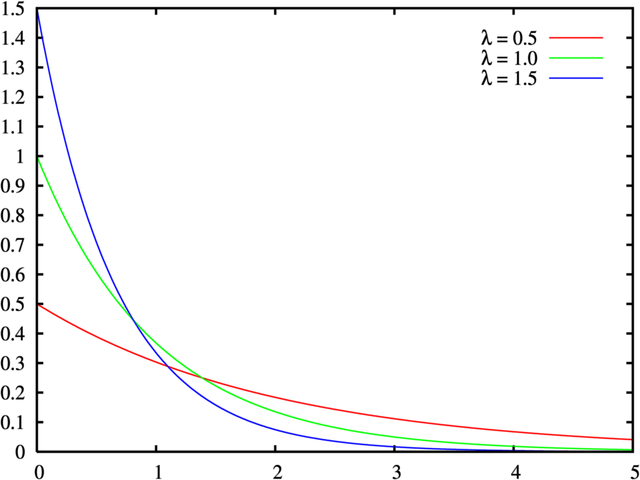
\includegraphics[scale = 0.3]{distribution_exponential}\\
  \caption{Exponential 概率密度函数}\label{fig.distribution.exponential}
\end{figure}
	
\textbf{累积分布函数}\\
累积分布函数可以写成:
$$F(x;\lambda )=\left\{{\begin{matrix}1-e^{{-\lambda x}}&,\;x\geq 0,\\0&,\;x<0.\end{matrix}}\right.$$
\begin{figure}[htbp]
  \centering
  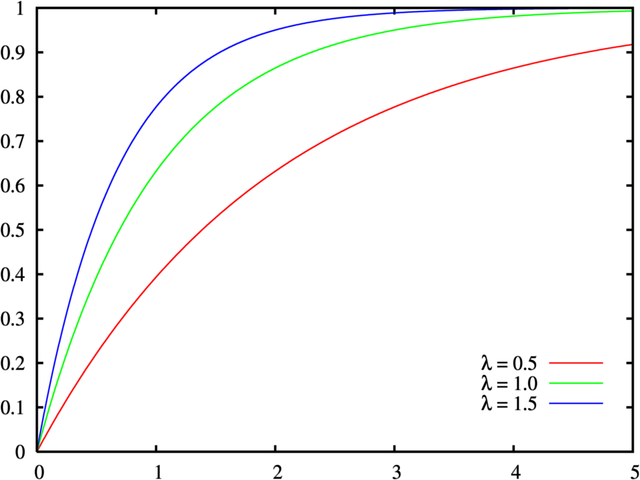
\includegraphics[scale = 0.3]{distribution_exponential_cdf}\\
  \caption{Exponential 累积分布函数}\label{fig.distribution.exponential.cdf}
\end{figure}
	
随机变量$X$ (概率参数是$\lambda$ ) 的期望值是:
$$
{\mathbf  {E}}[X]=\int_0^{\infty} xf(x)dx = {\frac  {1}{\lambda }}
$$
比方说:如果你平均每个小时接到2次电话,那么你预期等待每一次电话的时间是半个小时。
$X$ 的方差是:
$${\mathbf  {D}}[X]={\frac{1}{\lambda ^{2}}}
$$
$X$ 的偏离系数是: $V[X] = 1$

\textbf{与泊松过程的关系}\\
泊松过程是一种重要的随机过程。泊松过程中,第k次随机事件与第$k+1$次随机事件出现的时间间隔服从指数分布。这是因为,第$k$次随机事件之后长度为$t$的时间段内,第$k+1$次随机事件出现的概率等于$1$减去这个时间段内没有随机事件出现的概率。而根据泊松过程的定义,长度为$t$的时间段内没有随机事件出现的概率等于
$$
{\frac  {e^{{-\lambda t}}(\lambda t)^{0}}{0!}}=e^{{-\lambda t}}.
$$
所以第k次随机事件之后长度为t的时间段内,第$k+1$次随机事件出现的概率等于$1-e^{{-\lambda t}}$,这是指数分布。这还表明了泊松过程的无记忆性。

\section{Poisson分布}
\label{sec.distribution.poisson}
泊松分布适合于描述单位时间内随机事件发生的次数的概率分布。如某一服务设施在一定时间内受到的服务请求的次数,电话交换机接到呼叫的次数、汽车站台的候客人数、机器出现的故障数、自然灾害发生的次数、DNA序列的变异数、放射性原子核的衰变数等等。
泊松分布的概率质量函数为:
$$
P(X=k)={\frac  {e^{{-\lambda }}\lambda ^{k}}{k!}}
$$
泊松分布的参数$\lambda$ 是单位时间(或单位面积)内随机事件的平均发生率。
\begin{figure}[htbp]
  \centering
  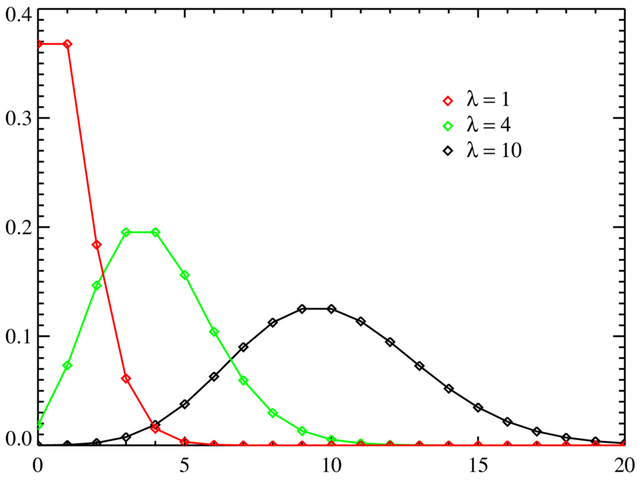
\includegraphics[scale = 0.3]{distribution_poisson}\\
  \caption{Poisson 概率分布}\label{fig.distribution.poisson}
\end{figure}

\begin{figure}[htbp]
  \centering
  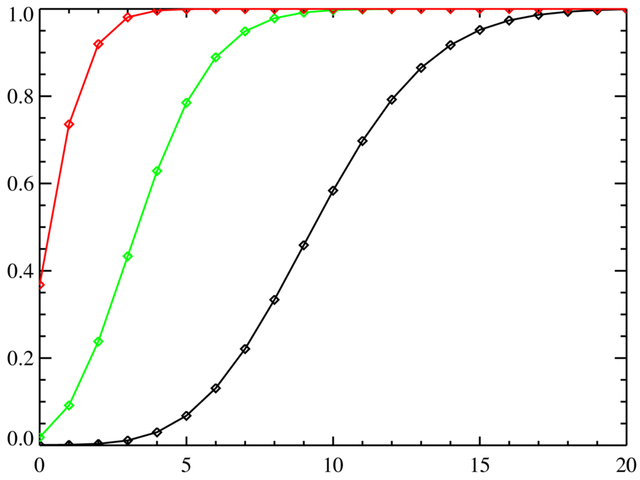
\includegraphics[scale = 0.3]{distribution_poisson_pmf}\\
  \caption{Poisson 累积分布函数}\label{fig.distribution.poisson.pmf}
\end{figure}
	
1.$E(X)=V(X)=\lambda$ \\
2.两个独立且服从泊松分布的随机变量,其和仍然服从泊松分布 (更精确地说:若$X \sim Poisson(\lambda_1)$且$Y \sim Poisson(\lambda_2)$,则 $X+Y \sim Poisson(\lambda_1+\lambda_2))$

\subsection{Poisson 分布与二项分布的关系}
%% http://my.oschina.net/u/347414/blog/129195
在二项分布的伯努利试验中,如果试验次数$n$很大,二项分布的概率$p$很小,且乘积$\lambda = n$ \\$p$比较适中,则事件出现的次数的概率可以用泊松分布来逼近。事实上,\textbf{二项分布可以看作泊松分布在离散时间上的对应物}。
\begin{proof}
证明如下。首先,回顾e的定义:
$$
\lim _{{n\to \infty }}\left(1-{\lambda  \over n}\right)^{n}=e^{{-\lambda }},
$$
二项分布的定义:
$$
P(X=k)={n \choose k}p^{k}(1-p)^{{n-k}}.
$$
如果令$p=\lambda /n$, $n$趋于无穷时$P$的极限:
$$
\begin{aligned}
\lim_{{n \to \infty }}P(X=k) & =\lim _{{n\to \infty }}{n \choose k}p^{k}(1-p)^{{n-k}}\\
& = \lim _{{n\to \infty }}{n! \over (n-k)!k!}\left({\lambda \over n}\right)^{k}\left(1-{\lambda \over n}\right)^{{n-k}}\\
& = \lim _{{n\to \infty }}\underbrace {\left[{\frac {n!}{n^{k}\left(n-k\right)!}}\right]}_{F}\left({\frac {\lambda ^{k}}{k!}}\right)\underbrace {\left(1-{\frac {\lambda }{n}}\right)^{n}}_{{\to \exp \left(-\lambda \right)}}\underbrace {\left(1-{\frac {\lambda }{n}}\right)^{{-k}}}_{{\to 1}}\\
& = \lim _{{n\to \infty }}\underbrace {\left[\left(1-{\frac {1}{n}}\right)\left(1-{\frac {2}{n}}\right)\ldots \left(1-{\frac {k-1}{n}}\right)\right]}_{{\to 1}}\left({\frac {\lambda ^{k}}{k!}}\right)\underbrace {\left(1-{\frac {\lambda }{n}}\right)^{n}}_{{\to \exp \left(-\lambda \right)}}\underbrace {\left(1-{\frac {\lambda }{n}}\right)^{{-k}}}_{{\to 1}}\\
& = \left({\frac {\lambda ^{k}}{k!}}\right)\exp \left(-\lambda \right)
\end{aligned}
$$
\end{proof}
\end{document}
